\documentclass[]{article}

\usepackage[utf8]{inputenc}
\usepackage{amsmath}
\usepackage{amssymb}
\usepackage{amsthm}
\usepackage{amsfonts}
\usepackage{graphicx}
\usepackage{capt-of}
\usepackage{listings}
\usepackage{siunitx}
\usepackage[section]{placeins}
\usepackage{float}



% Oppgavenummerering %
\renewcommand\thesection{Problem \arabic{section}}
\renewcommand\thesubsection{\alph{subsection})}

% Bevis
\newcommand\TombStone{\rule{.5em}{.5em}}
\renewcommand\qedsymbol{\TombStone}

\title{Adaptiv – Assignment 1}
\author{Sigurd Totland | MTTK}

\begin{document}
\maketitle

\section{}
The system is given as
\begin{equation}\begin{aligned}
\mathbf{\dot x} = \mathbf{Ax} + \mathbf{B}u.
\end{aligned}\end{equation}
This means we can use an estimation scheme of the form
\begin{equation}\begin{aligned}
\mathbf{\dot {\hat x}} = \mathbf{\hat A \hat x} + \mathbf{\hat B} u.
\end{aligned}\end{equation}
We define the estimation error as
\begin{equation}\begin{aligned}
\epsilon_1 \triangleq \mathbf{x} - \mathbf{\hat x}.
\end{aligned}\end{equation}
From equation (4.2.29) in I\&S we obtain a good update law for parameter estimation. These are
\begin{equation}\begin{aligned}
\mathbf{\dot {\hat A}} = \gamma_1 \epsilon_1 \mathbf{\hat x}^\top,
\quad \text{and} \quad
\mathbf{\dot {\hat B}} = \gamma_2 \epsilon_1 u^\top.
\end{aligned}\end{equation}
We simulate this scheme in matlab using the values given in the problem, with unit estimator gains $\gamma_1$ and $\gamma_2$ as well as initial conditions $\mathbf{\hat A}_0 = \mathbf{I}$, $\mathbf{\hat B}_0 = \mathbf{1}$ and $\mathbf{\hat x}_0=\mathbf{0}$. We have plotted in figures 1–6 both the $\mathbf{\hat A}$, $\mathbf{\hat B}$ and $\epsilon_1$ values for two different kinds of inputs, namely
\begin{equation}\begin{aligned}
u(t) = 10\sin(2t),
\quad \text{and} \quad
u(t) = 10\sin(2t) + 7\cos(3.6t).
\end{aligned}\end{equation}
We see that the first input, having only one sine function, isn't able to achieve convergence in the parameters, while the second one with two sines, is. A general rule of thumb for this kind of estimation scheme is that the more sine functions there are in the input signal, the more parameters can be estimated. In both cases however, the error $\epsilon_1$ goes to zero.
\begin{figure}[H]
\centering
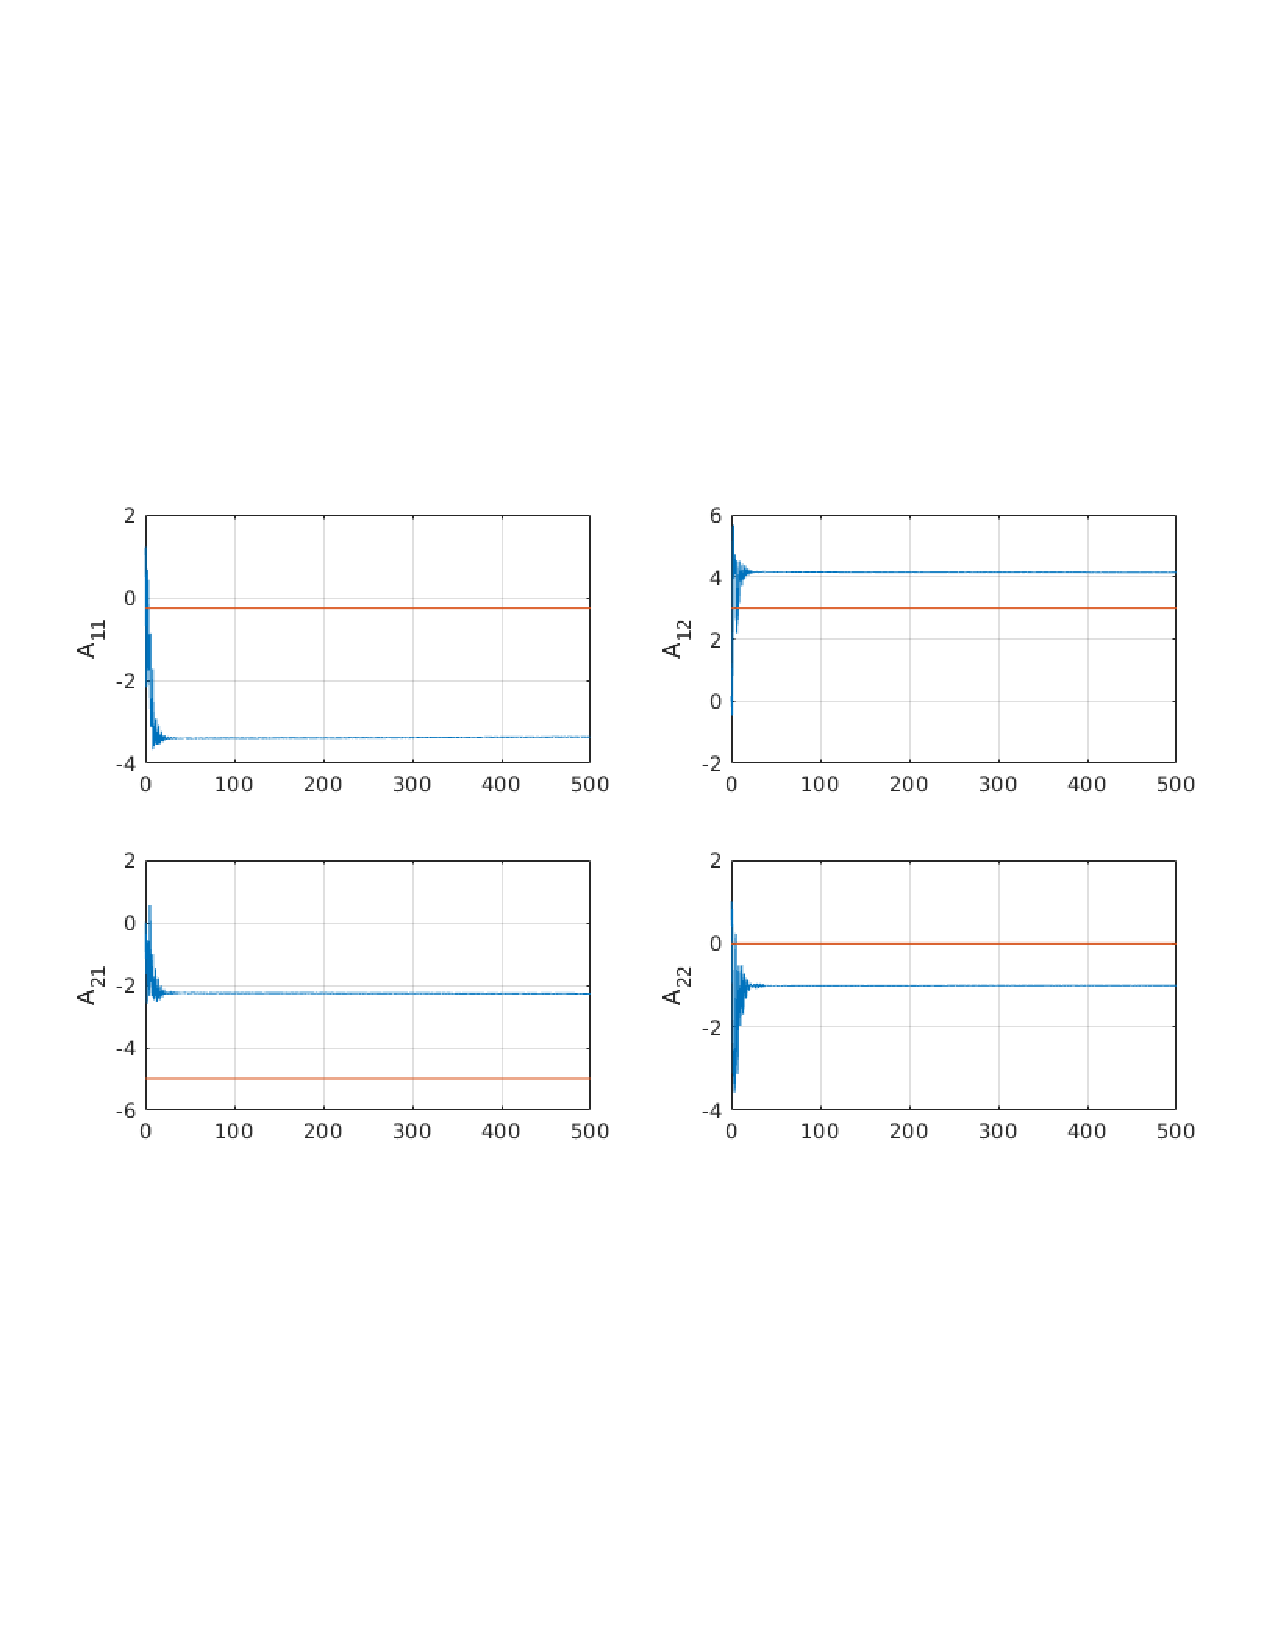
\includegraphics[width=1\columnwidth]{one_sine_A.pdf}
\caption{One sine function $\mathbf{\hat A}$}
\label{fig:one_sine_A}
\end{figure}
\begin{figure}[H]
\centering
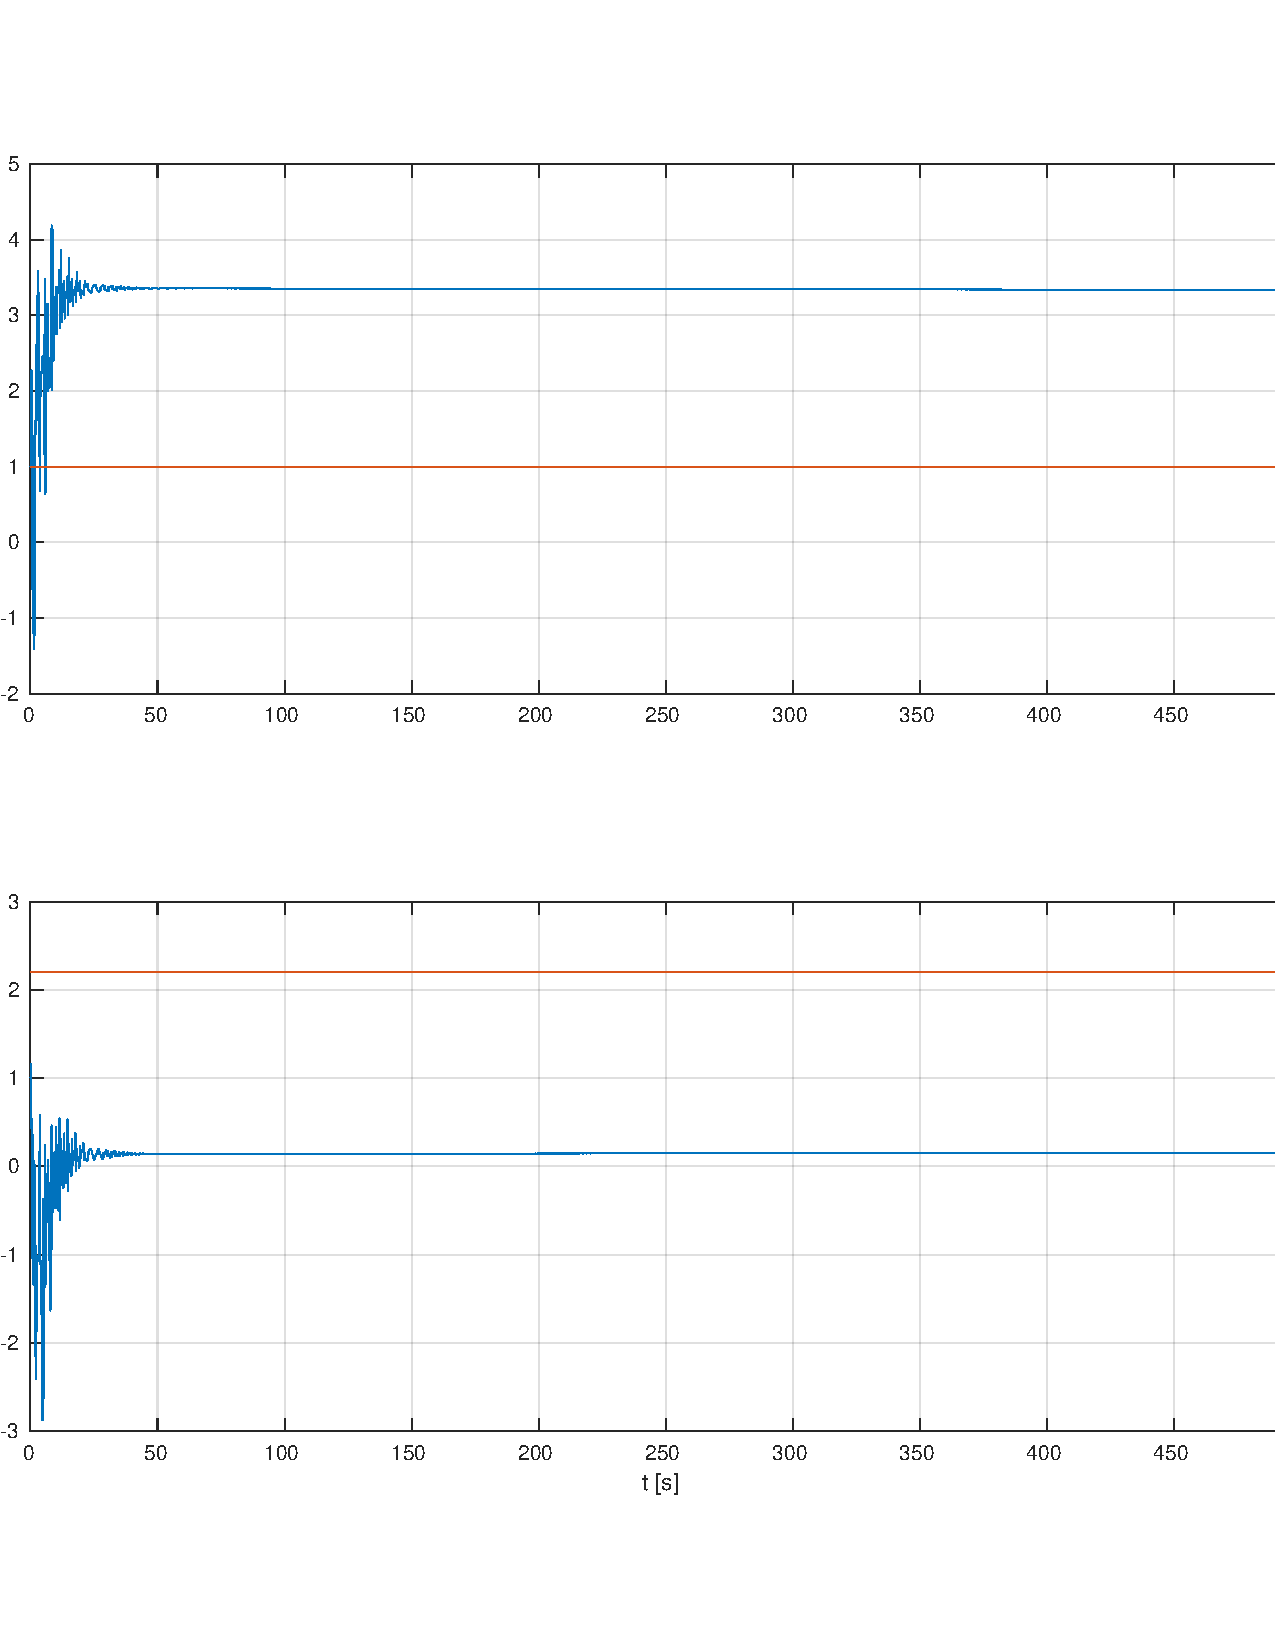
\includegraphics[width=1\columnwidth]{one_sine_B.pdf}
\caption{One sine function $\mathbf{\hat B}$}
\label{fig:one_sine_B}
\end{figure}
\begin{figure}[H]
\centering
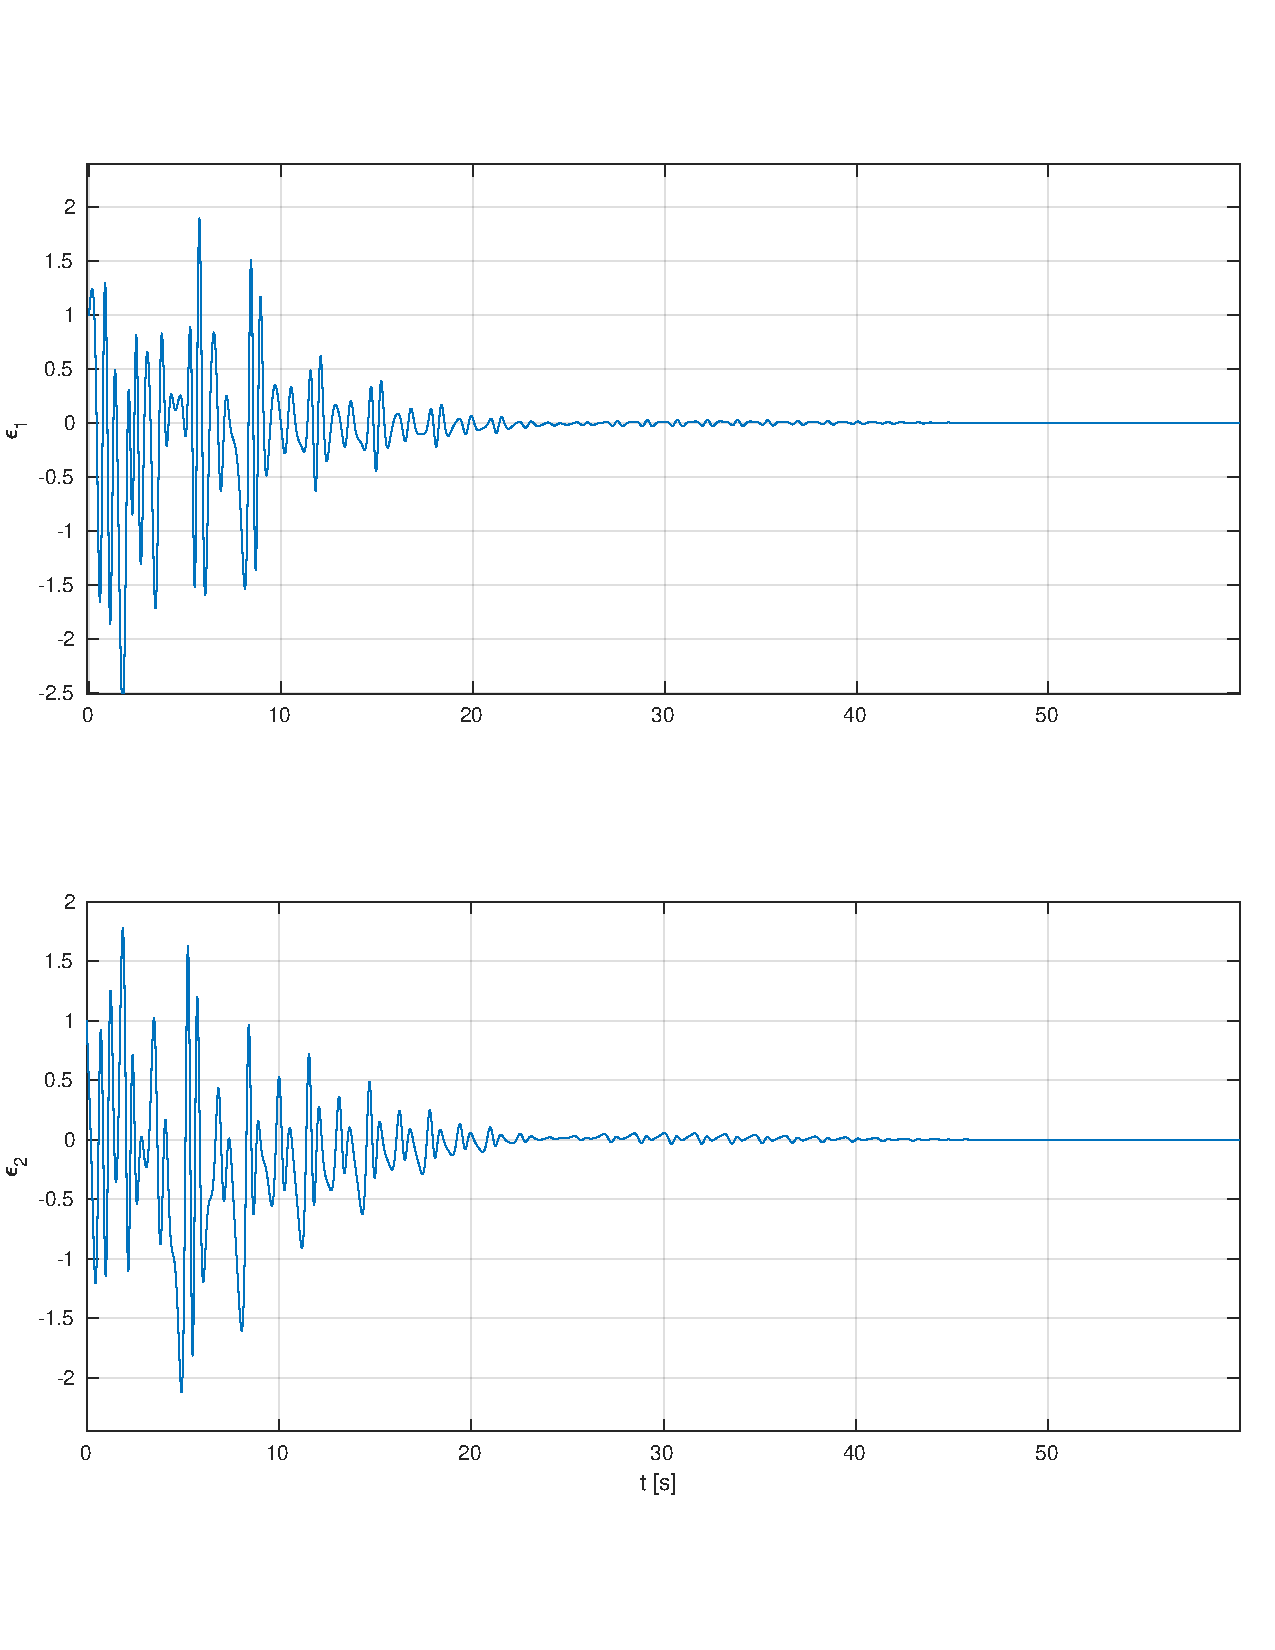
\includegraphics[width=1\columnwidth]{one_sine_error.pdf}
\caption{One sine function $\epsilon_1$}
\label{fig:one_sine_error}
\end{figure}
\begin{figure}[H]
\centering
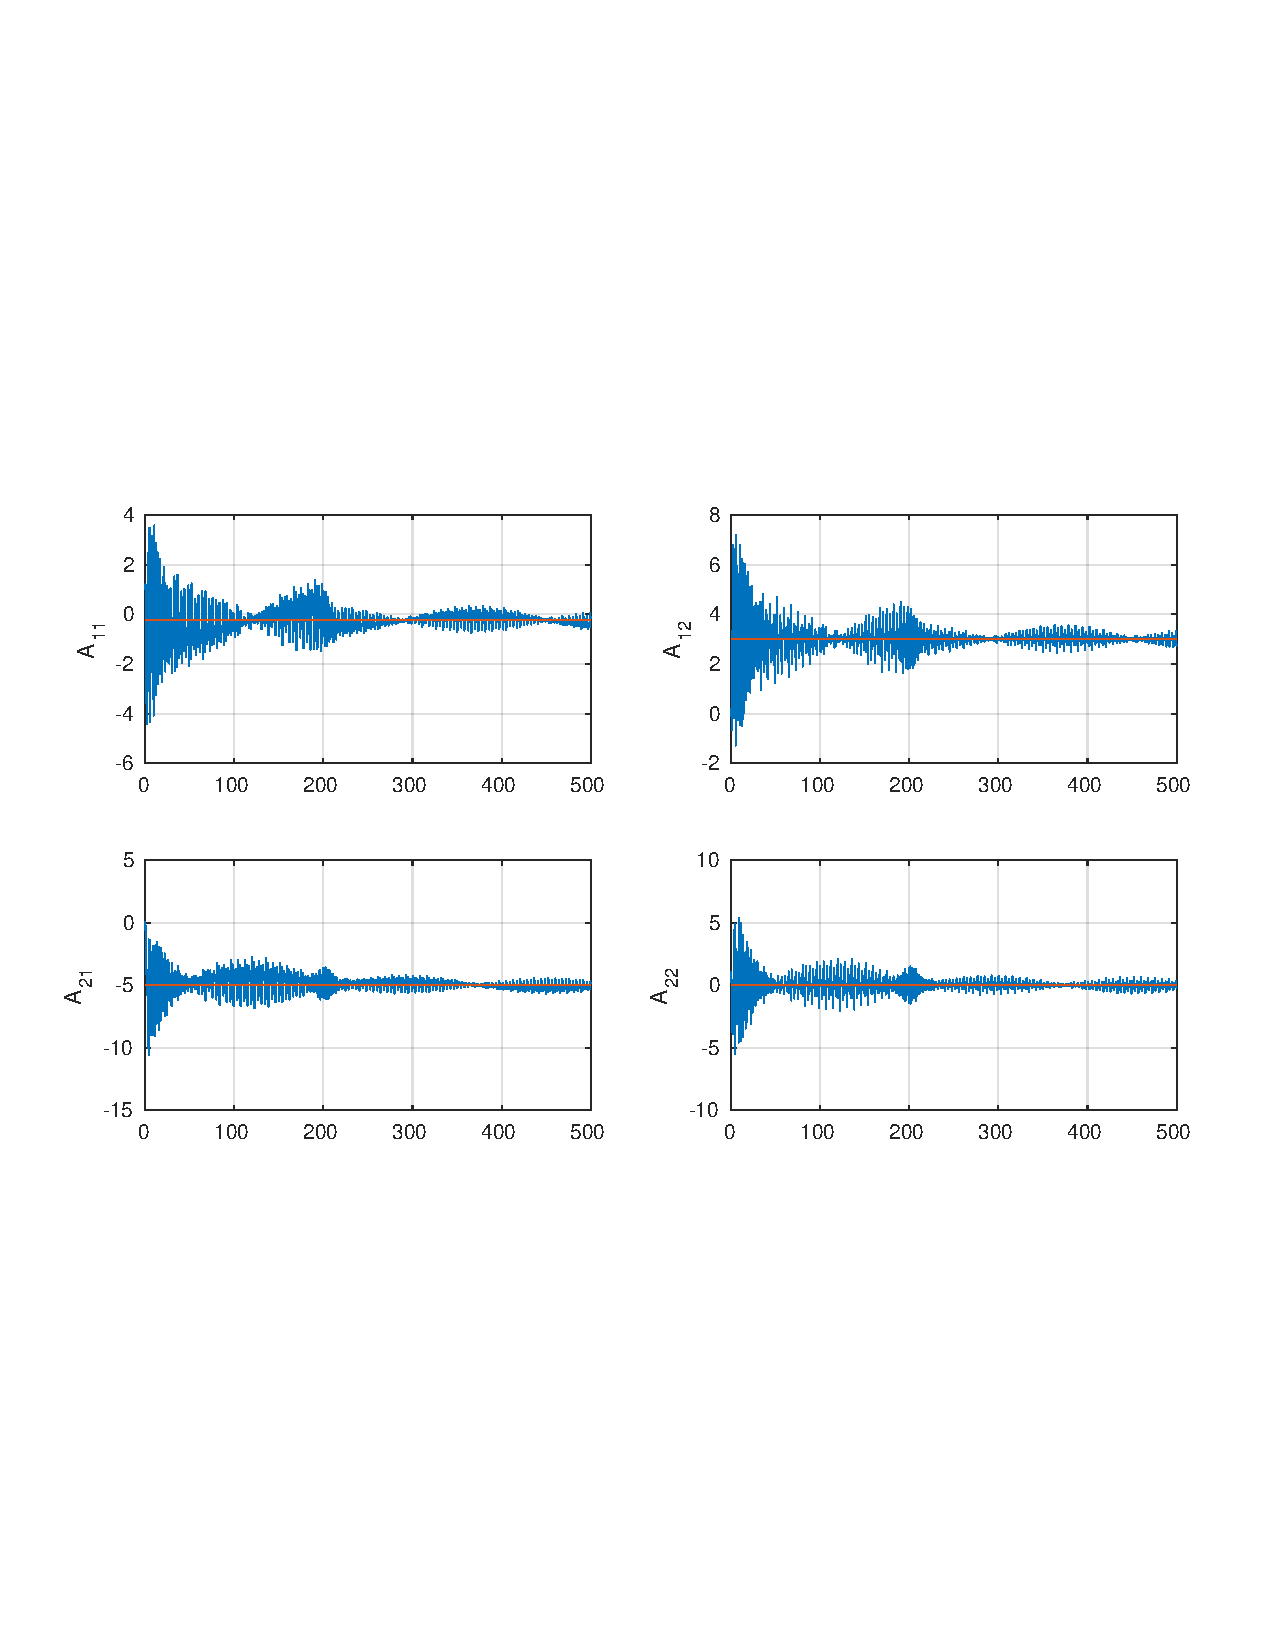
\includegraphics[width=1\columnwidth]{two_sine_A.pdf}
\caption{Two sine functions $\mathbf{\hat A}$}
\label{fig:two_sine_A}
\end{figure}
\begin{figure}[H]
\centering
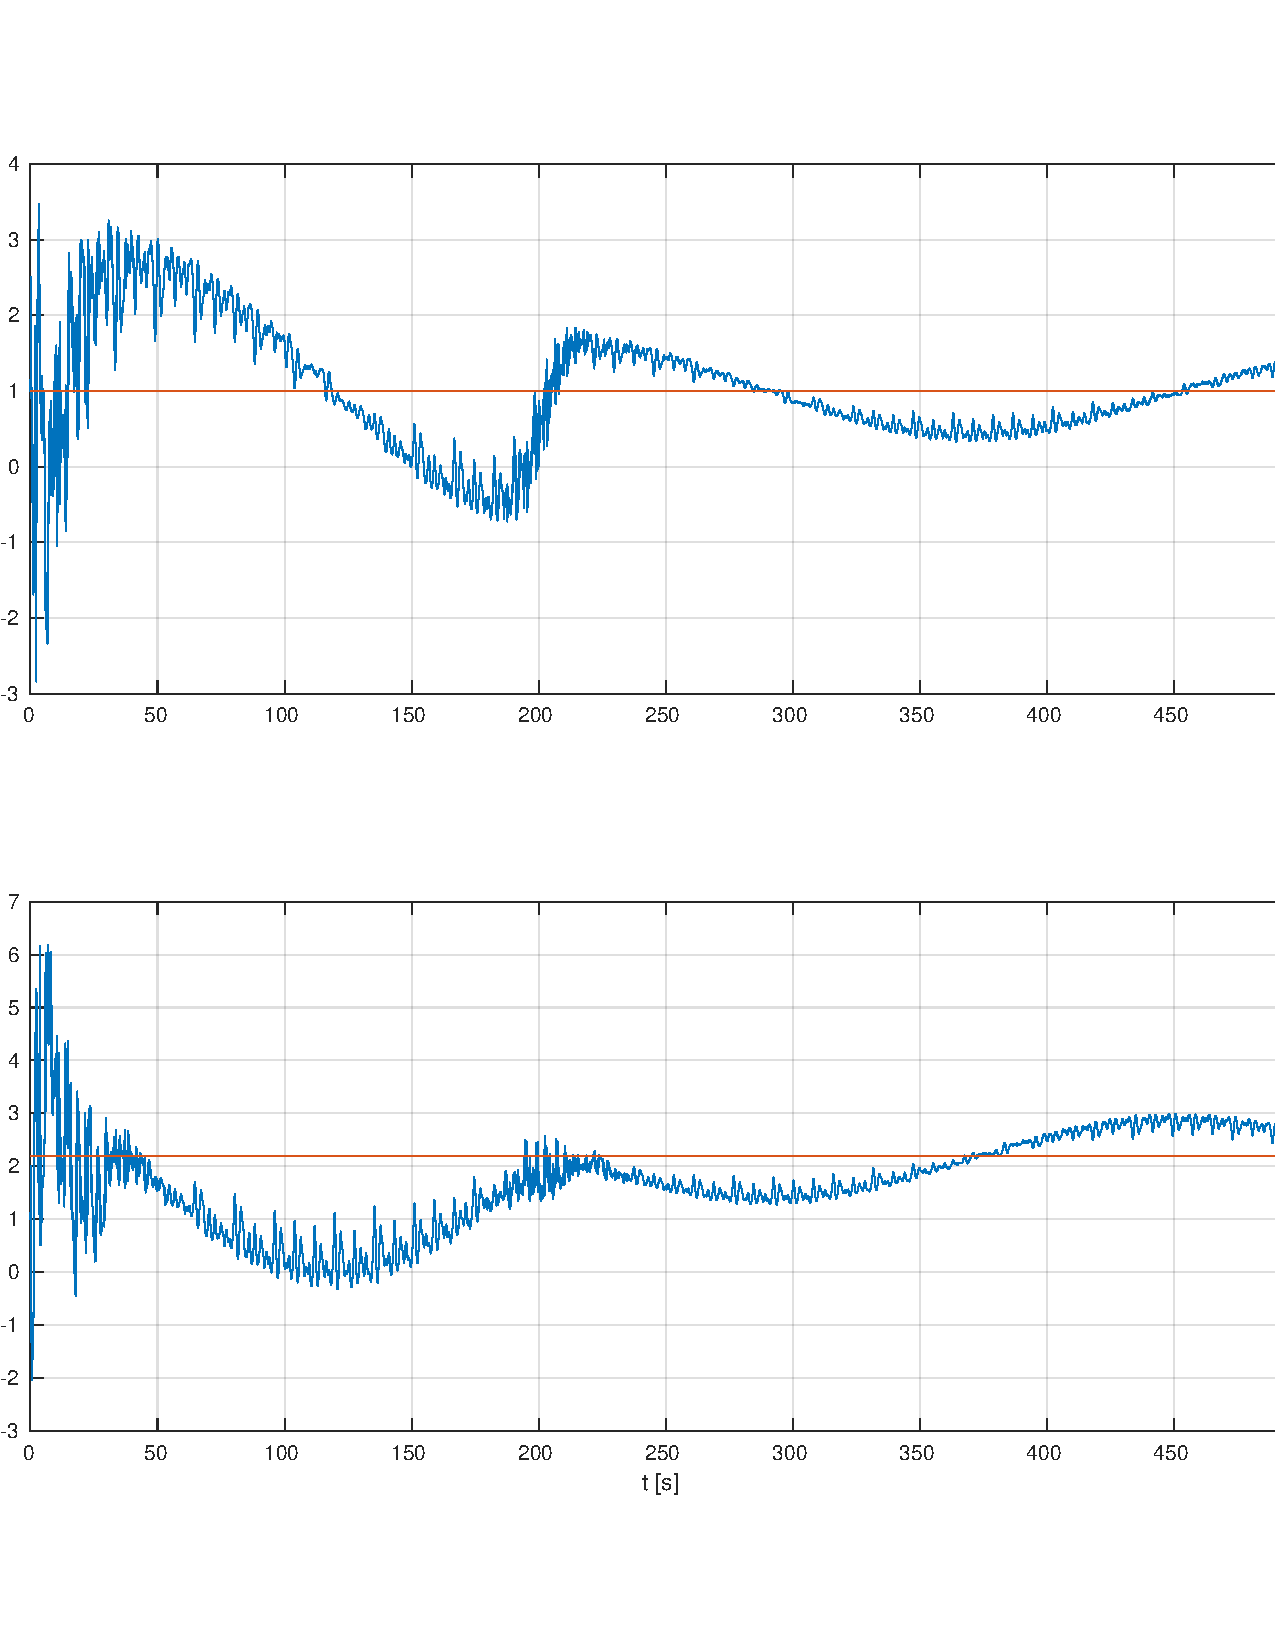
\includegraphics[width=1\columnwidth]{two_sine_B.pdf}
\caption{Two sine functions $\mathbf{\hat B}$}
\label{fig:two_sine_B}
\end{figure}
\begin{figure}[H]
\centering
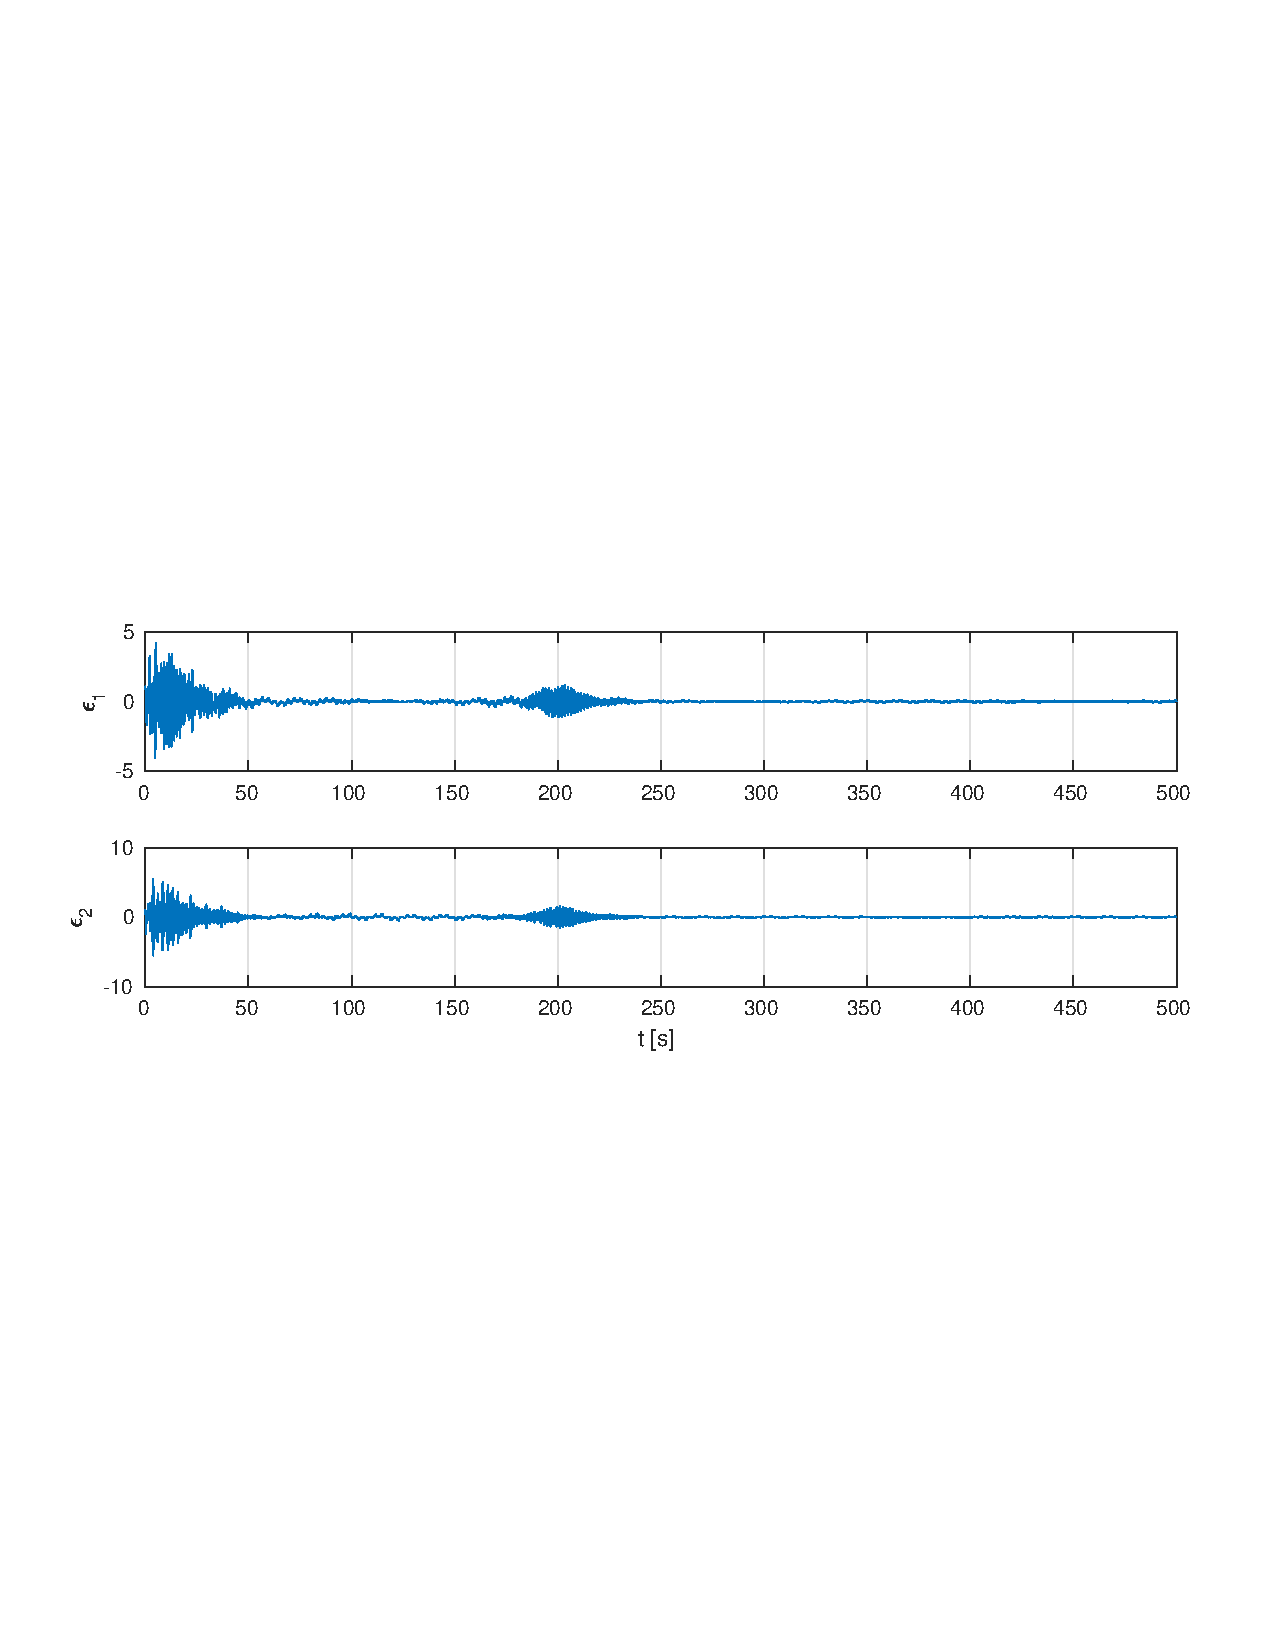
\includegraphics[width=1\columnwidth]{two_sine_error.pdf}
\caption{Two sine functions $\epsilon_1$}
\label{fig:two_sine_error}
\end{figure}

\section{I\&S P4.3}
The task is to find an adaptive law for estimating the parameters $a_i$ and $b_i$ on-line in the system
\begin{equation}\begin{aligned}
\dot x = a_1f_1(x)+a_2f_2(x)+b_1g_1(x)u+b_2g_2(x)u.
\end{aligned}\end{equation}
We begin by rewriting the system with $s$ as a differentiation operator obtaining
\begin{equation}\begin{aligned}
\label{eq:system_laplace}
s x = a_1F_1+a_2F_2+b_1G_1u+b_2G_2u.
\end{aligned}\end{equation}
We wish to rewrite this to the form of Equation (4.2.12) in I\&S, i.e. $y=\theta^{*\top} \phi$. For that, we first need to filter the left hand side of equation \eqref{eq:system_laplace} to make it proper. To do this, we define a filter $\Lambda(s)$ that is any Hurwitz polynomial in s of degree $\geq 1$. The filtered system becomes
\begin{equation}\begin{aligned}
\frac{s x}{\Lambda(s)} = \frac{a_1F_1+a_2F_2+b_1G_1u+b_2G_2u}{\Lambda(s)}.
\end{aligned}\end{equation}
We can write this as
\begin{equation}\begin{aligned}
z = \theta^{*\top}\phi
\end{aligned}\end{equation}
where
\begin{equation}\begin{aligned}
z = \frac{sx}{\Lambda(s)},
\end{aligned}\end{equation}
\begin{equation}\begin{aligned}
\theta^* =
\begin{bmatrix}
a_1 & a_2 & b_1 & b_2
\end{bmatrix}
\end{aligned}\end{equation}
are our unknown parameters, and
\begin{equation}\begin{aligned}
\phi =
\frac{1}{\Lambda(s)}
\begin{bmatrix}
F_1 \\
F_2 \\
G_1u \\
G_2u \\
\end{bmatrix}
\end{aligned}\end{equation}
are our known signals. We let $\theta$ denote the estimate of $\theta^*$ and obtain the estimate
\begin{equation}\begin{aligned}
\hat z = \theta^\top \phi
\end{aligned}\end{equation}
With this, we define the estimation error
\begin{equation}\begin{aligned}
\epsilon_1 = z - \hat z.
\end{aligned}\end{equation}
Inserting our expressions for $z$ and $\hat z$ and defining the parameter estimation error $\tilde \theta = \theta - \theta^*$, the above expression can be written
\begin{equation}\begin{aligned}
\epsilon_1 = z - \theta^\top \phi = \theta^{* \top} \phi - \theta^\top = -\tilde \theta^\top \phi.
\end{aligned}\end{equation}
Our final estimation scheme will then amount to a minimizer of this error expression. For that, we can for instance use the gradient method. We define the cost function
\begin{equation}\begin{aligned}
J(\theta) = \frac{\epsilon_1^2}{2} = \frac{(z - \theta^\top \phi)^2}{2}.
\end{aligned}\end{equation}
Our adaptive law then becomes
\begin{equation}\begin{aligned}
\dot \theta = -\Gamma \nabla J(\theta) = \Gamma(z - \theta^\top \phi)\phi = \Gamma \epsilon_1 \phi,
\quad \theta(0) = \theta_0,
\end{aligned}\end{equation}
where we have defined a symmetrical and positive definite matrix $\Gamma$ as the \textit{adaptive gain}.

\section{}
We begin by assuming that the infimum of $V$ exists and define
\begin{equation}\begin{aligned}
V_m = \inf_{t\geq 0}V(t).
\end{aligned}\end{equation}
We want to show that the limit $\lim_{t\rightarrow \infty}V(t)$ exists and is finite. Because $V$ is non-decreasing, in terms of the infimum, this is equivalent to showing that
\begin{equation}\begin{aligned}
\label{eq:infimum_limit}
\lim_{t \rightarrow \infty} V(t) = V_m.
\end{aligned}\end{equation}
For some $t > 0$ we define a $t' > 0$ such that $t \geq t'$. Because of the non-increasing property of $V$, we have that $V(t) \geq V(t')$. Using the infimum, we can rewrite this expression to one using an $\epsilon > 0$, i.e. $V(t) \geq V_m + \epsilon$. Furthermore, from the definition of the infimum, we know that $V_m \leq V(t), \forall t\geq 0$, thus we have shown that for arbitrarily large $t$, $V(t)$ gets arbitrarily close to $V_m$, or formally, $\forall \epsilon > 0, \exists t \geq 0 \text{ s.t. } V_m \leq V(t) \leq V_m + \epsilon$ and hence \eqref{eq:infimum_limit} holds. \qed


\section{}
From equation (4.2.10) in I\&S we have that the closed form solution to $\dot{ \tilde \theta} = -\gamma u^2 \tilde \theta$ is
\begin{equation}\begin{aligned}
\tilde \theta (t) = e^{-\gamma \int^{t}_{0}u^2(\tau)d \tau}\tilde \theta(0).
\end{aligned}\end{equation}
To show this is exponentially decreasing, we must ensure that it is bounded by an exponentially decreasing function, i.e.
\begin{equation}\begin{aligned}
\label{eq:exp_bound}
e^{-\gamma \int^{t}_{0}u^2(\tau)d \tau} \leq \alpha_1 e^{-\gamma_1 t}
\end{aligned}\end{equation}
for some $\alpha_1, \gamma_1 > 0$ and for all $t$. We have here assumed $\tilde \theta(0) < \infty$ as this is also necessary for convergence. To arrive at condition (4.2.11) in I\&S, we piece time into $n$ finite intervals of length $T_0$. This results in the integral in the exponent becoming
\begin{equation}\begin{aligned}
\label{eq:integral_sum}
\int^{t}_{0}u^2(\tau)d \tau = \sum_{k=1}^{n}\int^{kT_0}_{(k-1)T_0}u^2(\tau)d \tau  + \int^{t}_{nT_0}u^2(\tau)d \tau.
\end{aligned}\end{equation}
Note how the sum in \eqref{eq:integral_sum} is a constant in time. Using this knowledge, we rewrite equation \eqref{eq:exp_bound} to
\begin{equation}\begin{aligned}
e^{-\gamma \int^{t}_{0}u^2(\tau)d \tau} &= e^{-\gamma (\sum_{k=1}^{n}\int^{kT_0}_{(k-1)T_0}u^2(\tau)d \tau  + \int^{t}_{nT_0}u^2(\tau)d \tau)} \\
&= (\prod_{k=1}^n e^{-\gamma\int^{kT_0}_{(k-1)T_0}u^2(\tau)d \tau  }) e^{-\gamma\int^{t}_{nT_0}u^2(\tau)d \tau} \\
&\leq \alpha_1 e^{-\gamma_1 t} \\
&= \alpha_1 e^{-\gamma_1 nT_0}e^{-\gamma_1 (t - nT_0)}.
\end{aligned}\end{equation}
By introducing positive constants $t_1 = nT_0$, $\gamma_0 = \gamma$ and
\begin{equation}\begin{aligned}
\alpha = \frac{\alpha_1 e^{-\gamma_1 t_1}}{\prod_{k=1}^n e^{-\gamma\int^{kT_0}_{(k-1)T_0}u^2(\tau)d \tau  }}
\end{aligned}\end{equation}
the condition \eqref{eq:exp_bound} becomes
\begin{equation}\begin{aligned}
\label{eq:dumb_condition}
e^{-\gamma \int^{t}_{t_1}u^2(\tau)d \tau} \leq \alpha e^{-\gamma_0(t-t_1)}.
\end{aligned}\end{equation}
Informally this means that to show that $\tilde \theta$ decreases exponentially, we must only show that its \textit{tail} is bounded by an exponentially decreasing function. \\

We now consider condition (4.2.11). By defining
\begin{equation}\begin{aligned}
\alpha_0 = \frac{\gamma_0}{\gamma} - \frac{\ln \alpha}{\gamma T_0}
\end{aligned}\end{equation}
 we get
\begin{equation}\begin{aligned}
\label{eq:alpha}
\alpha = e^{\gamma_0 T_0 - \gamma \alpha_0 T_0}.
\end{aligned}\end{equation}
From \eqref{eq:dumb_condition} we have
\begin{equation}\begin{aligned}
e^{-\gamma\int^{t+T_0}_{t}u^2(\tau)d \tau} \leq \alpha e^{-\gamma_0(t+T_0-t)} = \alpha e^{-\gamma_0 T_0}.
\end{aligned}\end{equation}
Inserting \eqref{eq:alpha}, this becomes
\begin{equation}\begin{aligned}
\label{eq:cool_condition}
e^{-\gamma\int^{t+T_0}_{t}u^2(\tau)d \tau} \leq e^{-\gamma_0 T_0 + \gamma_0 T_0 - \gamma \alpha_0 T_0} = e^{ - \gamma \alpha_0 T_0}.
\end{aligned}\end{equation}
Hence,
\begin{equation}\begin{aligned}
\int^{t+T_0}_{t}u^2(\tau)d \tau \geq \alpha_0 T_0 \implies \eqref{eq:dumb_condition}.
\end{aligned}\end{equation}
To show that (4.2.11) $\iff$ \eqref{eq:dumb_condition}, we must also show that \eqref{eq:dumb_condition} $\implies$ (4.2.11). For this, we multiply $-\gamma$ on both sides of the equality in (4.2.11) obtaining
\begin{equation}\begin{aligned}
-\gamma \int^{t+T_0}_{t}u^2(\tau)d \tau \leq -\gamma \alpha_0 T_0.
\end{aligned}\end{equation}
Since the exponential function is monotonically increasing, we can take the exponent and preserve the inequality. This yields equation \eqref{eq:cool_condition}, i.e.
\begin{equation*}\begin{aligned}
e^{-\gamma \int^{t+T_0}_{t}u^2(\tau)d \tau} \leq e^{-\gamma \alpha_0 T_0}.
\end{aligned}\end{equation*}
From our logic above, we know that this can be rewritten to \eqref{eq:dumb_condition}, meaning that if (4.2.11) is satisfied, \eqref{eq:dumb_condition} is too, and (4.2.11) $\iff$ \eqref{eq:dumb_condition}. \qed
\end{document}

